\documentclass[a4paper,titlepage]{article}

% Se cargan los paquetes necesarios
\usepackage[spanish]{babel}
\usepackage[utf8]{inputenc}
\usepackage{graphicx}
\usepackage{helvet}
\usepackage[T1]{fontenc}
\usepackage{multirow}
\usepackage{listings}
\usepackage{verbatim}
\usepackage{indentfirst}
\usepackage{color}
\usepackage[x11names]{xcolor}
\usepackage{hyperref}
\usepackage{graphicx}
\usepackage{multirow}
\usepackage{eurosym}


\definecolor{dkgreen}{rgb}{0,0.6,0}
\definecolor{gray}{rgb}{0.5,0.5,0.5}
\definecolor{mauve}{rgb}{0.58,0,0.82}


\lstset{
  literate=
   {á}{{\'a}}1
   {í}{{\'i}}1
   {é}{{\'e}}1
   {ú}{{\'u}}1
   {ó}{{\'o}}1
   {Á}{{\'A}}1
   {Í}{{\'I}}1
   {É}{{\'E}}1
   {Ú}{{\'U}}1
   {Ó}{{\'O}}1
   {ñ}{{\~n}}1
   {Ñ}{{\~N}}1
   {€}{{\euro}}1
}

\lstset{
  frame=leftline,
  basicstyle=\footnotesize,       % the size of the fonts that are used for the code
  numbers=left,                   % where to put the line-numbers
  numberstyle=\tiny\color{gray},  % the style that is used for the line-numbers
  numbersep=5pt,                  % how far the line-numbers are from the code
  backgroundcolor=\color{white},  % choose the background color. You must add \usepackage{color}
  showspaces=false,               % show spaces adding particular underscores
  showstringspaces=false,         % underline spaces within strings
  showtabs=false,                 % show tabs within strings adding particular underscores
  rulecolor=\color{black},        % if not set, the frame-color may be changed on line-breaks within not-black text (e.g. comments (green here))
  tabsize=2,                      % sets default tabsize to 2 spaces
  captionpos=b,                   % sets the caption-position to bottom
  breaklines=true,                % sets automatic line breaking
  breakatwhitespace=false,        % sets if automatic breaks should only happen at whitespace
  title=\lstname,                 % show the filename of files included with \lstinputlisting;
                                  % also try caption instead of title
  keywordstyle=\color{blue},      % keyword style
  commentstyle=\color{dkgreen},   % comment style
  stringstyle=\color{mauve},      % string literal style
  escapeinside={(*@}{@*)},        % if you want to add LaTeX within your code
  morekeywords={*,},           % if you want to add more keywords to the set
  deletekeywords={...}            % if you want to delete keywords from the given language
}


\hypersetup{
  colorlinks=true,
  linkcolor=blue
}

\setlength{\abovecaptionskip}{2pt}

% type user-defined commands here

\renewcommand*{\lstlistlistingname}{Índice de Listings}


\begin{document}

\title{\Huge{Memoria da Práctica de ACS} \\ \small{Rede de Caixeros}}
\author{Pablo Castro Valiño \\ \small{(pablo.castro1@udc.es)} \and
Marcos Chavarría Teijeiro \\ \small{(marcos.chavarria@udc.es)}}
\date{2012-2013}
\maketitle

\tableofcontents

\newpage

\section{Decisiones de Diseño}
\subsection {FAP}
Para facer máis sinxelo a elaboración da practica creamos unha librería que permite crear mensaxes a partir do valor dos seus campos e a partir dun string co formato indicado. Isto permitenos reducir a complexidade de traballar con unha gran cantidade de mensaxes con diferentes formatos. Ademais creamos test de unidade para comprobar que non existisen erros nesta parte da práctica.

\subsection {Banco}
Para implementar a interación entre interface e base de datos intentouse empregar un patrón MVC de forma que a interface esta a espera de que se lle avise de cambios producidos na base de datos.

Para programar os diferentes estados nos que se pode atopar o banco empregouse un patrón estado de forma que se delega a acción a realizar nunha clase estado que a súa vez chama con uns parametros determinados a unha funcion da clase Banco.

\subsection {Consorcio}
\subsection {Caixeiro}
\newpage

\clearpage
\newpage


\section {Bases de datos}
\subsection {Banco}

\begin{figure}[h!]
  \begin{center}
    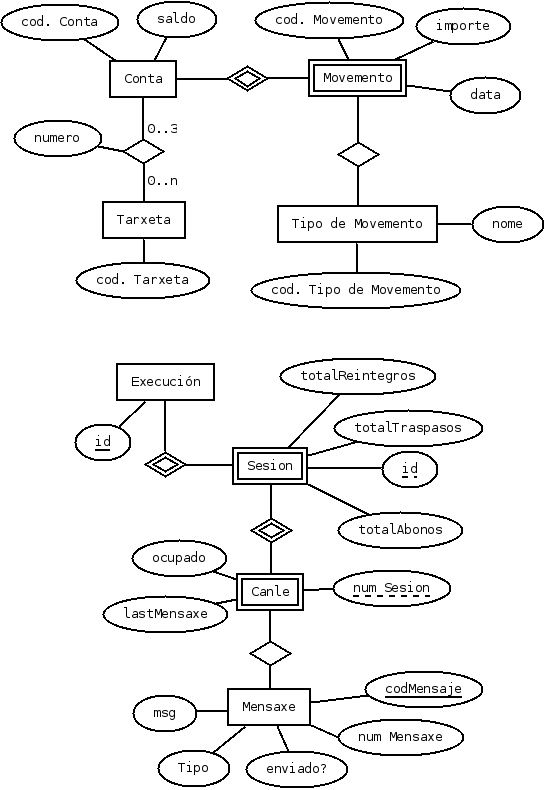
\includegraphics[width=0.9\textwidth]{diagrama_bd_bancos.png}
  \end{center}
\end{figure}

\lstinputlisting[language=SQL]{creacion_bd_bancos.sql}

\clearpage

\subsection {Consorcio}

\begin{figure}[h!]
  \begin{center}
    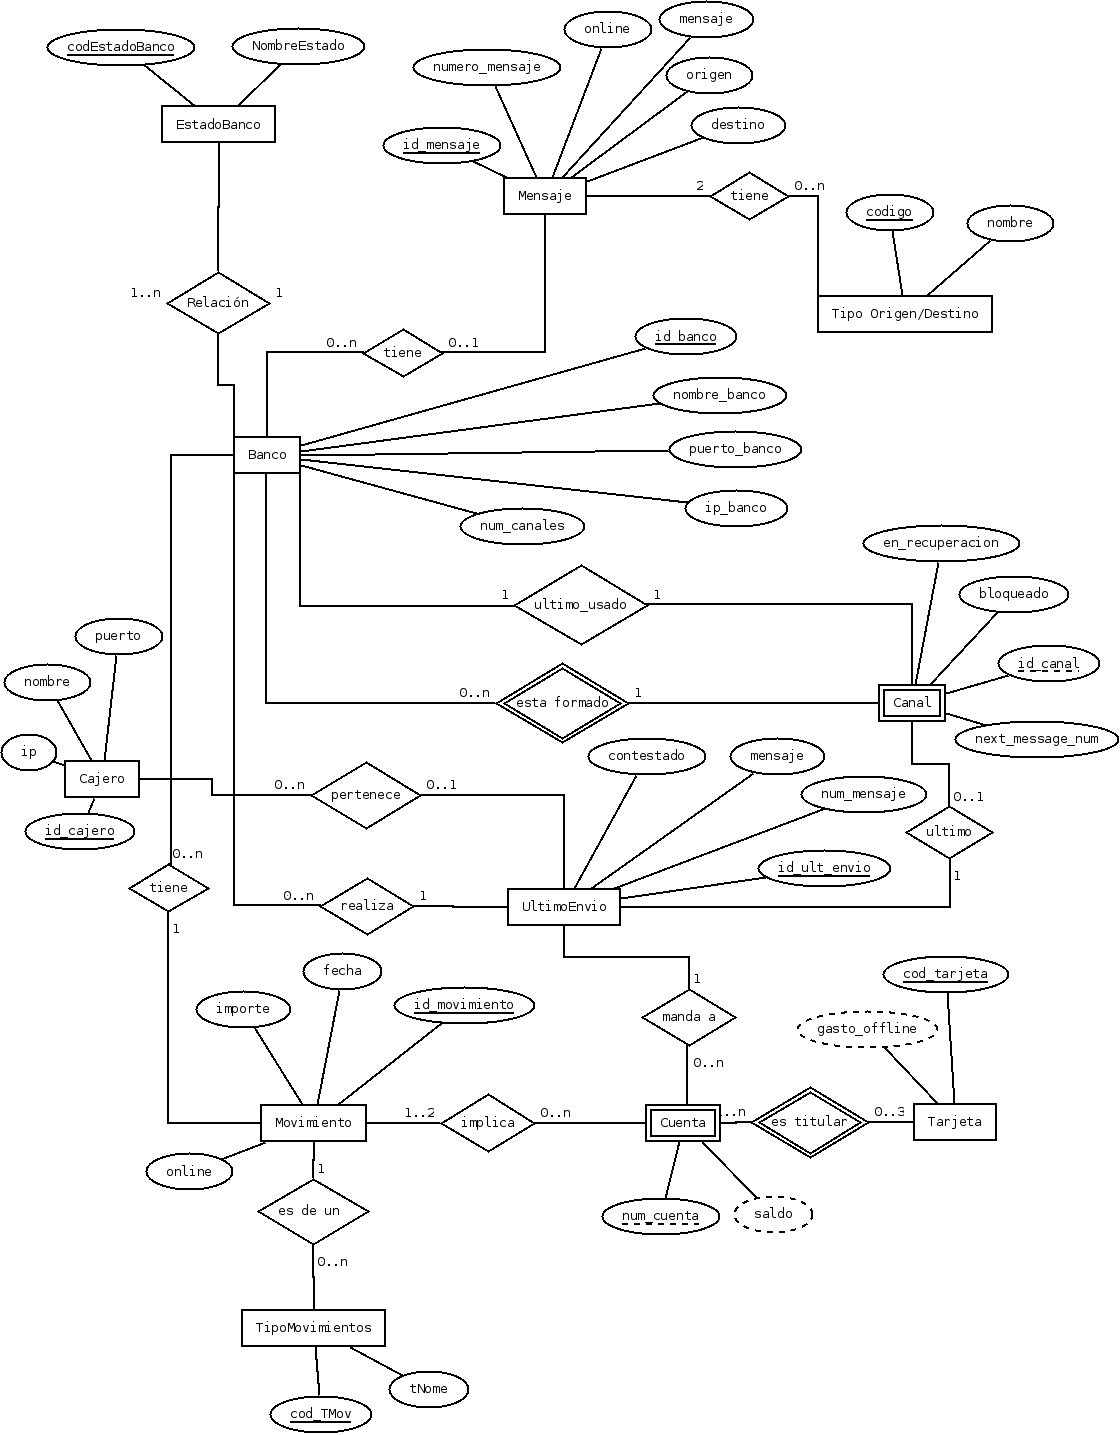
\includegraphics[width=0.9\textwidth]{diagrama_bd_consorcio.png}
  \end{center}
\end{figure}

\lstinputlisting[language=SQL]{creacion_bd_consorcio.sql}

\clearpage
\newpage

\section {Diagramas UML}

\clearpage
\newpage

\section {Codigo Fonte}
\subsection{Banco}
\subsubsection{Aplicativo}
\lstinputlisting[language=Java]{../src/practicaacs/AppBanco.java}
\subsubsection{Clase Banco}
\lstinputlisting[language=Java]{../src/practicaacs/banco/Banco.java}
\subsubsection{Canal}
\lstinputlisting[language=Java]{../src/practicaacs/banco/bd/Canal.java}
\subsubsection{ClineteBDBanco}
\lstinputlisting[language=Java]{../src/practicaacs/banco/bd/ClienteBDBanco.java}
\subsubsection{Conta}
\lstinputlisting[language=Java]{../src/practicaacs/banco/bd/Conta.java}
\subsubsection{Mensaxe}
\lstinputlisting[language=Java]{../src/practicaacs/banco/bd/Mensaxe.java}
\subsubsection{Movemento}
\lstinputlisting[language=Java]{../src/practicaacs/banco/bd/Movemento.java}
\subsubsection{Tarxeta}
\lstinputlisting[language=Java]{../src/practicaacs/banco/bd/Tarxeta.java}
\subsubsection{AnalizadorMensajes}
\lstinputlisting[language=Java]{../src/practicaacs/banco/csconsorcio/AnalizadorMensajes.java}
\subsubsection{ClienteServidorConsorcio}
\lstinputlisting[language=Java]{../src/practicaacs/banco/csconsorcio/ClienteServidorConsorcio.java}
\subsubsection{EstadoSesion}
\lstinputlisting[language=Java]{../src/practicaacs/banco/estados/EstadoSesion.java}
\subsubsection{Sesión Aberta}
\lstinputlisting[language=Java]{../src/practicaacs/banco/estados/SesAberta.java}
\subsubsection{Sesión Detida}
\lstinputlisting[language=Java]{../src/practicaacs/banco/estados/SesDetida.java}
\subsubsection{Sesión Non Aberta}
\lstinputlisting[language=Java]{../src/practicaacs/banco/estados/SesNonAberta.java}
\subsubsection{Sesión en Recuperación}
\lstinputlisting[language=Java]{../src/practicaacs/banco/estados/SesRecuperacion.java}
\subsubsection{Sesión con Solicitude de Apertura}
\lstinputlisting[language=Java]{../src/practicaacs/banco/estados/SolApertura.java}
\subsubsection{Sesión con Solicitude de Deter Tráfico}
\lstinputlisting[language=Java]{../src/practicaacs/banco/estados/SolDeter.java}
\subsubsection{Sesión con Solicitude de Pechar Sesión}
\lstinputlisting[language=Java]{../src/practicaacs/banco/estados/SolPechar.java}
\subsubsection{Sesión con Solicitude de Reanudar Tráfico}
\lstinputlisting[language=Java]{../src/practicaacs/banco/estados/SolReanudar.java}
\subsubsection{Diálogo Abrir Sesión}
\lstinputlisting[language=Java]{../src/practicaacs/banco/iu/DialogoAbrirSesion.java}
\subsubsection{Diálogo Error}
\lstinputlisting[language=Java]{../src/practicaacs/banco/iu/DialogoError.java}
\subsubsection{Diálogo Nova Conta Asociada}
\lstinputlisting[language=Java]{../src/practicaacs/banco/iu/DialogoNovaContaAsociada.java}
\subsubsection{Diálogo Nova Conta}
\lstinputlisting[language=Java]{../src/practicaacs/banco/iu/DialogoNovaConta.java}
\subsubsection{Diálogo Nova Tarxeta}
\lstinputlisting[language=Java]{../src/practicaacs/banco/iu/DialogoNovaTarxeta.java}
\subsubsection{Diálogo Si ou Non}
\lstinputlisting[language=Java]{../src/practicaacs/banco/iu/DialogoSiNon.java}
\subsubsection{Ventana Banco}
\lstinputlisting[language=Java]{../src/practicaacs/banco/iu/VentanaBanco.java}


\subsection{Caixeiro}
\subsubsection{Aplicación}
\lstinputlisting[language=Java]{../src/practicaacs/AppCajero.java}
\subsubsection{Cajeto}
\lstinputlisting[language=Java]{../src/practicaacs/cajeros/Cajero.java}
\subsubsection{Conexion}
\lstinputlisting[language=Java]{../src/practicaacs/cajeros/ConexionCajero.java}
\subsubsection{Envio}
\lstinputlisting[language=Java]{../src/practicaacs/cajeros/Envio.java}
\subsubsection{Consulta Abstracta}
\lstinputlisting[language=Java]{../src/practicaacs/cajeros/iu/ConsultaAbstracta.java}
\subsubsection{Interface de Usuario Consulta de Movimientos}
\lstinputlisting[language=Java]{../src/practicaacs/cajeros/iu/ConsultarMovimientos_IU.java}
\subsubsection{Interface de Usuario Consulta Saldo}
\lstinputlisting[language=Java]{../src/practicaacs/cajeros/iu/ConsultarSaldo_IU.java}
\subsubsection{Interface de Usuario Pantalla Inicial}
\lstinputlisting[language=Java]{../src/practicaacs/cajeros/iu/PantallaInicialCajero_IU.java}
\subsubsection{Interface de Usuario Realizar Abono}
\lstinputlisting[language=Java]{../src/practicaacs/cajeros/iu/RealizarAbono_IU.java}
\subsubsection{Interface de Usuario Realizar Reintegro}
\lstinputlisting[language=Java]{../src/practicaacs/cajeros/iu/RealizarReintegro_IU.java}
\subsubsection{Interface de Usuario Realizar Traspaso}
\lstinputlisting[language=Java]{../src/practicaacs/cajeros/iu/RealizarTraspaso_IU.java}
\subsubsection{Interface de Usuario Seleción Acción}
\lstinputlisting[language=Java]{../src/practicaacs/cajeros/iu/SeleccionAccion_IU.java}


\subsection{Consorcio}
\subsubsection{Aplicación}
\lstinputlisting[language=Java]{../src/practicaacs/AppConsorcio.java}
\subsubsection{Consorcio}
\lstinputlisting[language=Java]{../src/practicaacs/consorcio/Consorcio.java}
\subsubsection{Conexión Consorcio-Caixeiro}
\lstinputlisting[language=Java]{../src/practicaacs/consorcio/ConexionConsorcio_Cajeros.java}
\subsubsection{Conexión Consorcio-Banco}
\lstinputlisting[language=Java]{../src/practicaacs/consorcio/ConexionConsorcio_Bancos.java}
\subsubsection{Servidor Consorcio-Banco}
\lstinputlisting[language=Java]{../src/practicaacs/consorcio/ServidorConsorcio_Bancos.java}
\subsubsection{Servidor Consorcio-Caixeiro}
\lstinputlisting[language=Java]{../src/practicaacs/consorcio/ServidorConsorcio_Cajeros.java}
\subsubsection{Estado Envio}
\lstinputlisting[language=Java]{../src/practicaacs/consorcio/aux/EstadoEnvio.java}
\subsubsection{Mensaje Cajero}
\lstinputlisting[language=Java]{../src/practicaacs/consorcio/aux/MensajeCajero.java}
\subsubsection{Movimiento}
\lstinputlisting[language=Java]{../src/practicaacs/consorcio/aux/Movimiento.java}
\subsubsection{Sesión}
\lstinputlisting[language=Java]{../src/practicaacs/consorcio/aux/Sesion.java}
\subsubsection{Tipo de Acción}
\lstinputlisting[language=Java]{../src/practicaacs/consorcio/aux/TipoAccion.java}
\subsubsection{Tipo Origen/Destino}
\lstinputlisting[language=Java]{../src/practicaacs/consorcio/aux/TipoOrigDest.java}
\subsubsection{Excepción BD Consorcio}
\lstinputlisting[language=Java]{../src/practicaacs/consorcio/bd/ConsorcioBDException.java}
\subsubsection{Librería Base de Datos}
\lstinputlisting[language=Java]{../src/practicaacs/consorcio/bd/Database_lib.java}
\subsubsection{Interface de Usuario Acerca De}
\lstinputlisting[language=Java]{../src/practicaacs/consorcio/iu/Acerca_de_IU.java}
\subsubsection{Interface Fin de Recuperación}
\lstinputlisting[language=Java]{../src/practicaacs/consorcio/iu/FinRecuperacion_IU.java}
\subsubsection{Interface Mostrar BD}
\lstinputlisting[language=Java]{../src/practicaacs/consorcio/iu/MostrarBD_IU.java}
\subsubsection{Pantalla Inicio Consorcio}
\lstinputlisting[language=Java]{../src/practicaacs/consorcio/iu/PantallaInicialConsorcio_IU.java}
\subsubsection{Interface Solicitude de Recuperación}
\lstinputlisting[language=Java]{../src/practicaacs/consorcio/iu/SolRecuperacion_IU.java}

\subsection{FAP}

\subsubsection{Excepción Código Non Valido}
\lstinputlisting[language=Java]{../src/practicaacs/fap/CodigoNoValidoException.java}
\subsubsection{Codigos de Error}
\lstinputlisting[language=Java]{../src/practicaacs/fap/CodigosError.java}
\subsubsection{Códigos de Mensaxes}
\lstinputlisting[language=Java]{../src/practicaacs/fap/CodigosMensajes.java}
\subsubsection{Códigos de Movemento}
\lstinputlisting[language=Java]{../src/practicaacs/fap/CodigosMovimiento.java}
\subsubsection{Códigos de Respuesta}
\lstinputlisting[language=Java]{../src/practicaacs/fap/CodigosRespuesta.java}
\subsubsection{Mensaje de Datos}
\lstinputlisting[language=Java]{../src/practicaacs/fap/MensajeDatos.java}
\subsubsection{Mensaje}
\lstinputlisting[language=Java]{../src/practicaacs/fap/Mensaje.java}
\subsubsection{Excepción Mensaje No Valido}
\lstinputlisting[language=Java]{../src/practicaacs/fap/MensajeNoValidoException.java}
\subsubsection{Mensaje Respuesta de Datos}
\lstinputlisting[language=Java]{../src/practicaacs/fap/MensajeRespDatos.java}
\subsubsection{Resposta Abono Erronea}
\lstinputlisting[language=Java]{../src/practicaacs/fap/RespAbonoError.java}
\subsubsection{Resposta Abono}
\lstinputlisting[language=Java]{../src/practicaacs/fap/RespAbono.java}
\subsubsection{Resposta Apertura Sesión}
\lstinputlisting[language=Java]{../src/practicaacs/fap/RespAperturaSesion.java}
\subsubsection{Resposta Cierre Sesión}
\lstinputlisting[language=Java]{../src/practicaacs/fap/RespCierreSesion.java}
\subsubsection{Resposta Datos Error}
\lstinputlisting[language=Java]{../src/practicaacs/fap/RespDatosError.java}
\subsubsection{Resposta Detencion Tráfico}
\lstinputlisting[language=Java]{../src/practicaacs/fap/RespDetTrafico.java}
\subsubsection{Resposta Fin de Tráfico en Recuperación}
\lstinputlisting[language=Java]{../src/practicaacs/fap/RespFinTraficoRec.java}
\subsubsection{Resposta Inicio de Tráfico en Recuperación}
\lstinputlisting[language=Java]{../src/practicaacs/fap/RespIniTraficoRec.java}
\subsubsection{Resposta Movementos Erronea}
\lstinputlisting[language=Java]{../src/practicaacs/fap/RespMovimientosError.java}
\subsubsection{Resposta Movementos}
\lstinputlisting[language=Java]{../src/practicaacs/fap/RespMovimientos.java}
\subsubsection{Resposta Reanudación Tráfico}
\lstinputlisting[language=Java]{../src/practicaacs/fap/RespReanTrafico.java}
\subsubsection{Resposta Reintegro Erroneo}
\lstinputlisting[language=Java]{../src/practicaacs/fap/RespReintegroError.java}
\subsubsection{Resposta Reintegro}
\lstinputlisting[language=Java]{../src/practicaacs/fap/RespReintegro.java}
\subsubsection{Resposta Saldo Erroneo}
\lstinputlisting[language=Java]{../src/practicaacs/fap/RespSaldoError.java}
\subsubsection{Resposta Saldo}
\lstinputlisting[language=Java]{../src/practicaacs/fap/RespSaldo.java}
\subsubsection{Resposta Traspaso Erroneo}
\lstinputlisting[language=Java]{../src/practicaacs/fap/RespTraspasoError.java}
\subsubsection{Resposta Traspaso}
\lstinputlisting[language=Java]{../src/practicaacs/fap/RespTraspaso.java}
\subsubsection{Resposta Abono}
\lstinputlisting[language=Java]{../src/practicaacs/fap/SolAbono.java}
\subsubsection{Solicitude Apertura de Sesión}
\lstinputlisting[language=Java]{../src/practicaacs/fap/SolAperturaSesion.java}
\subsubsection{Solicitude Peche de Sesión}
\lstinputlisting[language=Java]{../src/practicaacs/fap/SolCierreSesion.java}
\subsubsection{Solicitude Detención do Trafico}
\lstinputlisting[language=Java]{../src/practicaacs/fap/SolDetTrafico.java}
\subsubsection{Solicitude Fin Tráfico en Recuperación}
\lstinputlisting[language=Java]{../src/practicaacs/fap/SolFinTraficoRec.java}
\subsubsection{Solicitude Inicio Tráfico en Recuperación}
\lstinputlisting[language=Java]{../src/practicaacs/fap/SolIniTraficoRec.java}
\subsubsection{Solicitude Movementos}
\lstinputlisting[language=Java]{../src/practicaacs/fap/SolMovimientos.java}
\subsubsection{Solicitude Reanudar Tráfico}
\lstinputlisting[language=Java]{../src/practicaacs/fap/SolReanTrafico.java}
\subsubsection{Solicitude Reintegro}
\lstinputlisting[language=Java]{../src/practicaacs/fap/SolReintegro.java}
\subsubsection{Solicitude Saldo}
\lstinputlisting[language=Java]{../src/practicaacs/fap/SolSaldo.java}
\subsubsection{Solicitude Traspaso}
\lstinputlisting[language=Java]{../src/practicaacs/fap/SolTraspaso.java}

\clearpage
\newpage

\section{Arquivos de Configuración}
\subsection{Banco}
\lstinputlisting{../res/banco1.properties}

\subsection{Caixeiro}
\lstinputlisting{../res/cajero1.properties}

\subsection{Consorcio}
\lstinputlisting{../res/consorcio.properties}



\end{document}
